\section{Kostenarten}
Kalkulationen benötigt bestimmte eindeutige Kostenarten, die dann in einem Kostenartenplan aufgestellt und in einer Kostenartenrechnung kontrolliert werden können. Die eindeutige Kostenarten können in Kostenartenkategorien bzw. Kostenartengruppen zusammen fließen.  Im folgenden soll einmal festgehalten werden, was man für die Kalkulation nutzen sollte.

\begin{figure}[h!]
	\centering
	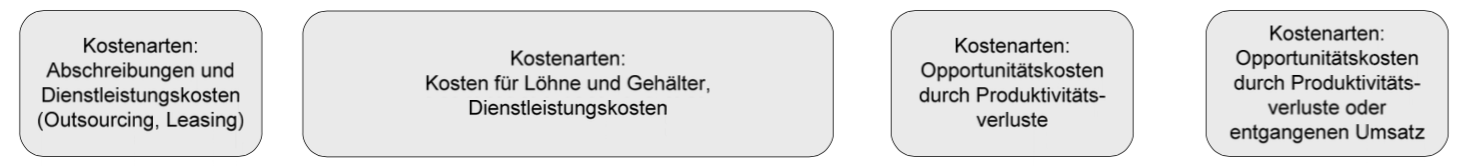
\includegraphics[width=10cm]{kapitel/gruppe4_2/bilder/beispiel_kostenarten_TCO}
	\caption{Beispiel von Kostenarten in der TCO-Methode, Grafik von Hansen}
	\label{fig_kostenarten_TCO}
\end{figure}

In der Abbildung \ref{fig_kostenarten_TCO} nach Hansen\footnote{\cite{hansen_business_2009}} finden sich z.B. in der von Krcmar benannten TCO-Methode (“Total Cost of Ownership”) wieder. Aus den bewerteten Daten der Kostenarten können periodische Durchschnittswerte ermittelt werden, aus denen dann für die Zukunft neue Abschätzungen gewonnen werden.

In einer ABC-Analyse kann eine weitere Klassifizierung vorgenommen werden, um z.B. aufzuzeigen welche Kostenarten auf jeden Fall (A-Klasse) anfallen, welche im besten Fall noch erledigt werden sollen (B-Klasse) und welche man optional (C-Klasse) aufwenden sollte.

Die Kostenarten der \ref{tab_gliederung_kostenarten} sind die Grundelemente der Wertsteigerung durch Wertschöpfung, die in die Kostenartenrechnung fließen sollten. „Die Kostenartenrechnung erfasst, systematisiert und periodisiert die Kosten.“\footnote{\cite{reim_erfolgsrechnung_2015}} 

Die Kostenarten der \ref{tab_gliederung_kostenarten} sollen in diesem Projekt als Übersicht dienen, da aktuell nur drei Module in der Kostenschätzung betrachtet werden, für den Fall das weitere Module abzuschätzen sind.

\begin{center}
	\label{tab_gliederung_kostenarten}
\begin{tabular}{|l|l|}
	\hline Gliederungsmerkmale nach  &  Kostenartengruppen\\ 
	\hline  &  \\ 
	\hline  &  \\ 
	\hline  &  \\ 
	\hline  &  \\ 
	\hline  &  \\ 
	\hline  &  \\ 
	\hline 
\end{tabular}
\end{center}